As a first step in the evaluation of our grammar-guided evolutionary search method, we consider two PDE-based model problems, Poisson's equation and a linear elastic boundary value problem, which can already be solved efficiently through iterative application of common multigrid cycles .
Here, our goal is, first of all, to demonstrate that our approach is able to reliably find functioning multigrid solvers in a number of randomized independent experiments.
Furthermore, since the known multigrid cycles already provide a strong baseline for these problems, we can investigate whether the methods evolved by our approach are able to achieve a similarly high degree of efficiency.
In addition, by considering both two and three-dimensional problems as well as a system of PDEs, we can demonstrate that our implementation is able to handle PDEs of different type.
\section{Evolving Monolithic Multigrid Solvers}
As it has been mentioned above, the goal of this section is to evaluate the effectiveness of our evolutionary search method in evolving multigrid methods that can be used as a standalone method for the numerical solution of a given PDE.
Therefore, the problem instances considered in this section are chosen in a way that facilitates their efficient solution by multigrid.
This is reflected in the fact that common multigrid cycles, as described in Section~\ref{sec:multigrid-cycles}, are able to quickly converge to the correct solution of each of the resulting systems of linear equations.
We begin this section by introducing the considered problem instances and their mathematical formulation. 
\subsection{Poisson's Equation}
\label{sec:poisson-equation}
Poisson's equation is an elliptic PDE that occurs in the study of many physical phenomena~\cite{folland2020introduction} and is defined as
\begin{equation}
	\begin{split}
		-\nabla^{2} u & = f \quad \text{in} \; \Omega \\
		u & = g \quad \text{on} \; \partial \Omega.
	\end{split}
	\label{eq:poisson}
\end{equation}
In our experimental evaluation, we consider two different instances of Poisson's equation with Dirichlet boundary conditions, which are summarized in Table~\ref{table:poisson-problems}.
\begin{table}
	\begin{tabular}{r l l}
		\toprule
		Problem & 2D Poisson & 3D Poisson \\
		\midrule
		$\Omega = $ & $ (0, 1)^2$ & $(0, 1)^3$ \\
		\midrule
		$f(\mathbf{x}) = $ & $\pi^2 \cos(\pi x) - 4 \pi^2 \sin(2 \pi y)$ & $x^2 - 0.5 y^2 - 0.5 z^2$ \\
		\midrule
		$g(\mathbf{x}) = $ & $\cos(\pi x) - \sin(\pi y)$ & $0$ \\
		\bottomrule
	\end{tabular}
	\caption{Poisson problem instances.}
	\label{table:poisson-problems}
\end{table}
Note that in Section~\ref{sec:execution-time-analysis} we have utilized the same two-dimensional instance of Poisson's equation to estimate the relative cost of each operation within our evolutionary search method.
We discretize the Laplace operator $\nabla^{2}$ with finite differences on a uniform cartesian grid with step size $h = 1/2^{l_{max}}$.
As a consequence, we obtain the five point stencil
\begin{equation*}
	\nabla^2_h = 
	\frac{1}{h^2} \begin{bmatrix}
		0 & 1 & 0\\
		1 & -4 & 1 \\
		0 & 1 & 0  
	\end{bmatrix},
\end{equation*}
in two dimensions and the seven point stencil
\begin{equation*}
\nabla^2_h = 
\frac{1}{h^2} \begin{bmatrix}
	\begin{bmatrix}
	0 & 0 & 0 \\
	0 & 1 & 0 \\
	0 & 0 & 0
	\end{bmatrix}
	&		
	\begin{bmatrix}
	0 & 1 & 0 \\
	1 & -6 & 1 \\
	0 & 1 & 0 
	\end{bmatrix} &
	\begin{bmatrix}
	0 & 0 & 0 \\
	0 & 1 & 0 \\
	0 & 0 & 0
\end{bmatrix}
\end{bmatrix}
\end{equation*} in three dimensions.
We choose a maximum level of $l_{max} = 11$ in 2D and $l_{max} = 7$ in 3D, which yields systems of linear equations consisting of $4\,190\,209$ and $2\,048\,383$ unknowns, respectively.

\subsection{Linear Elasticity}
Linear elasticity is a fundamental branch of solid mechanics with numerous applications in engineering and material science~\cite{holzapfel2001nonlinear}.
It simplifies the more general theory of nonlinear continuum mechanics by assuming a linear relationship between stress and strain during elastic deformation.
We consider a two-dimensional linear elastic boundary value problem given by the system of PDEs
\begin{equation}
	\begin{split}
		(\alpha + \beta) \cdot (\frac{\partial^2}{\partial x^2} u + \frac{\partial^2}{\partial x \partial y} v) + \alpha \nabla^2 u & = 0 \quad \text{in} \; \Omega \\
		(\alpha + \beta) \cdot (\frac{\partial^2}{\partial x \partial y} u + \frac{\partial^2}{\partial y^2} v) + \alpha \nabla^2 v & = 0 \quad \text{in} \; \Omega \\
		u = 0 \quad \text{and} \quad v & = g \quad \text{on} \; \partial \Omega 
		\label{eq:linear-elasticity}
	\end{split}
\end{equation}
where $\Omega = (0,1)^2$, $\alpha = 195$, $\beta = 130$ and
\begin{equation*}
	g(x,y) = 0.4 \, (1 - x) \, x y \, \sin(\pi x).
\end{equation*}
From a physical point of view, this system can be interpreted as a two-dimensional rectangular body that undergoes an elastic deformation into y-direction, as it can be seen in Figure~\ref{fig:visualization-linear-elasticity}.
\begin{figure}
	\centering
	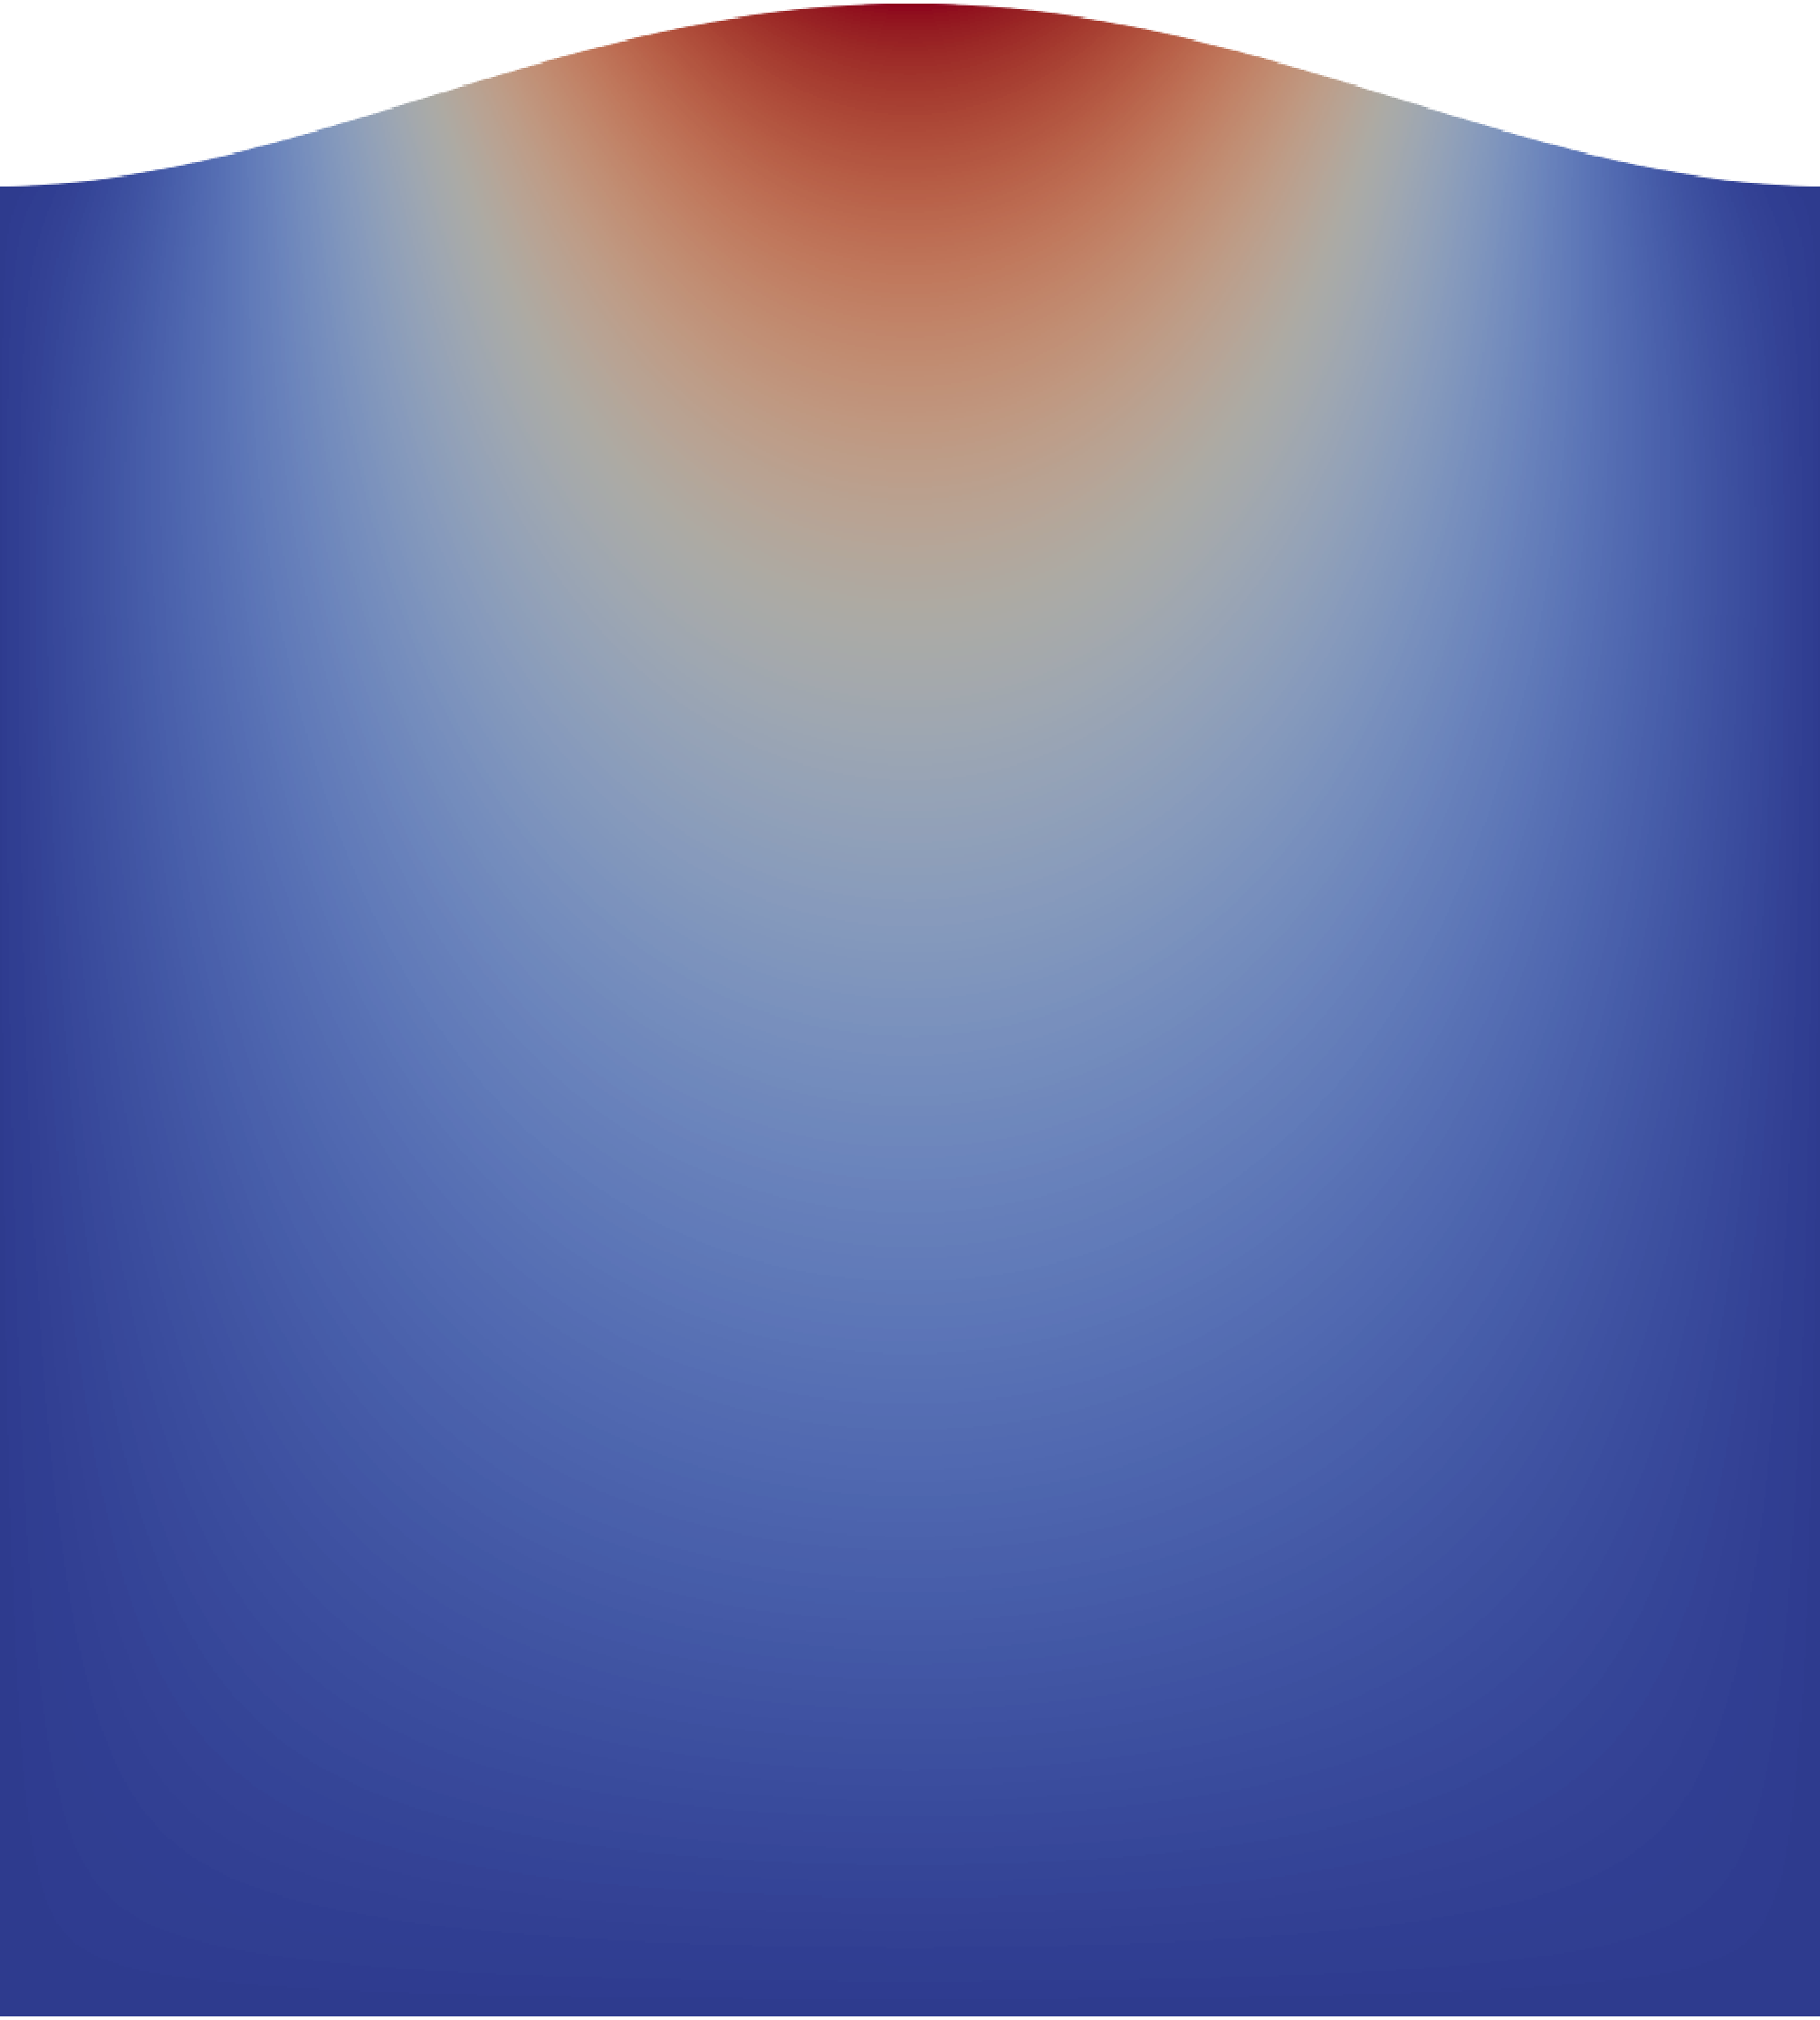
\includegraphics[width=0.5\textwidth]{figures/visualization-linear-elasticity1}
	\caption{Visualization of the considered linear elastic boundary value problem. A two-dimensional rectangular body undergoes an elastic deformation into y-direction.}
	\label{fig:visualization-linear-elasticity}
\end{figure}
We discretize equation \eqref{eq:linear-elasticity} with finite differences on a cartesian grid using a step size $h = 1/2^{l_{max}}$ with $l_{max} = 10$, which yields a system of linear equations $\boldsymbol{A} \boldsymbol{u} = \boldsymbol{f}$ with 
\begin{equation*}
	\boldsymbol{A} =
	\begin{pmatrix}
		(\alpha + \beta) \frac{\partial^2}{\partial x^2} + \alpha \nabla^2 & (\alpha + \beta) \frac{\partial^2}{\partial x \partial y} \\
		(\alpha + \beta) \frac{\partial^2}{\partial x \partial y} & (\alpha + \beta) \frac{\partial^2}{\partial y^2} +  \alpha \nabla^2
	\end{pmatrix},
\end{equation*}
\begin{equation*}
	\boldsymbol{u} = \begin{pmatrix}
		u \\ v
	\end{pmatrix}, \quad
	\boldsymbol{f} =
	\begin{pmatrix}
		f_{u} \\ f_{v}
	\end{pmatrix} =
	\begin{pmatrix}
		0 \\ 0
	\end{pmatrix},
\end{equation*}
whereby the differential operators $\nabla^2$, $\frac{\partial^2}{\partial x^2}$, $\frac{\partial^2}{\partial y^2}$ and $\frac{\partial^2}{\partial x \partial y}$ are approximated by their discrete counterparts
\begin{equation*}
	\left(\nabla^2 u\right)_{i,j} = 
	\frac{1}{h^2} \begin{bmatrix}
		0 & 1 & 0\\
		1 & -4 & 1 \\
		0 & 1 & 0  
	\end{bmatrix},
\end{equation*}
\begin{equation*}
	\left(\frac{\partial^2}{\partial x^2} u\right)_{i,j} =
		\frac{1}{h^2} \begin{bmatrix}
		0 & 0 & 0\\
		1 & -2 & 1 \\
		0 & 0 & 0  
	\end{bmatrix},
\end{equation*}
\begin{equation*}
	\left(\frac{\partial^2}{\partial y^2} u\right)_{i,j} =
	\frac{1}{h^2} \begin{bmatrix}
		0 & 1 & 0\\
		0 & -2 & 0 \\
		0 & 1 & 0  
	\end{bmatrix},
\end{equation*}
\begin{equation*}
	\left(\frac{\partial^2}{\partial x \partial y} u\right)_{i,j} = 
	\frac{1}{4 h^2} \begin{bmatrix}
		-1 & 0 & 1\\
		0 & 0 & 0 \\
		1 & 0 & -1  
	\end{bmatrix}.
\end{equation*}
Similar to the above case, we employ a uniform cartesian grid of size $h = 1/l_{max}$ with $l_{max} = 10$, such that the resulting system of linear equations contains $2\,093\,058$ unknowns.
\subsection{Multigrid Configuration}
To design a multigrid method, we consider each of the given problems a grid hierarchy consisting of five discretization levels $l \in \left[l_{max} - 4, l_{max}\right]$, where the grid spacing on each level is given by the formula $h = 1/2^l$.
We then obtain the respective operator on each level by applying the same discretization method as described above.
Therefore, the resulting grammar is structurally similar to the one in shown Table~\ref{table:multigrid-grammar}.
Within each grammar production rule, we then consider the following components:
\begin{description}
	\item[\textbf{Smoothers}:] Decoupled / Collective Jacobi and red-black Gauss-Seidel, block Jacobi with rectangular blocks up to a maximum number of 6 terms.
	\item[\textbf{Restriction}:] Full-weighting restriction.
	\item[\textbf{Prolongation}:] Bilinear interpolation.
	\item[\textbf{Relaxation factors}:] $\omega \in \left( 0.1 + 0.05i \right)_{i = 0}^{36} = \left(0.1, 0.15, 0.2, \dots 1.9 \right)$
	\item[\textbf{Coarse-grid solver}:] Conjugate gradient method for $l = l_{max} - 4$.
\end{description}
Here, we generate block Jacobi smoothers by defining a splitting $A = L + D + U$ where $D$ is a block diagonal matrix of the form
\begin{equation*}
	D = 
		\begin{pmatrix}A_{11}&0&\cdots &0\\
			0&A_{22}&\cdots &0\\
			\vdots &\vdots &\ddots &\vdots \\0&0&\cdots &A_{mm}\end{pmatrix},
\end{equation*}
where each matrix $A_{ij}$ corresponds to a set of adjacent grid points contained in the respective rectangular block, as it has been discussed in Section~\ref{subsec:block-smoothing}.
A more detailed treatment of block relaxation methods, can be found in~\cite{trottenberg2000multigrid}.
For each of smoothing and coarse-grid correction step the relaxation factor $\omega$ is chosen from the above sequence.
As a baseline for assessing the efficiency and generalizability of the evolved multigrid solvers, we consider a number of common multigrid cycles with red-black Gauss-Seidel smoothing and optimized relaxation factors.
We, therefore, formulate these methods on the same five-grid hierarchy, whereby we also utilize the same restriction, prolongation operators and coarse-grid solver, as described above.
\subsection{Optimization Settings and Evaluation Platform}
After specifying the operator and parameter choices considered within the construction of each multigrid solver, we next describe the settings under which we perform each GP-based optimization run.
Here, we utilize the EvoStencils framework, whose implementation has been described in detail in Chapter~\ref{chapter:evostencils-1} and~\ref{chapter:evostencils-2}.
The goal of each optimization run is then to evolve the set of non-dominated according to the two objectives convergence factor and execution time per iteration, as described in Section~\ref{sec:fitness-evaluation-and-selection}, which are evaluated by applying each multigrid method as an iterative solver to the respective test problem.
The resulting individuals are then subject to a subsequent evaluation and comparison with the available reference methods. 
Table~\ref{table:gp-parameters} gives an overview about the configuration of the EvoStencils framework used within each experiment.
\begin{table}
	\centering
	\caption{Summary of GGGP configuration parameters.}
	\label{table:gp-parameters}
	\begin{tabular}{l c}
		\toprule
		Parameter & Value \\
		\midrule 
		Evolutionary algorithm type & $(\mu + \lambda)$ \\
		\midrule
		Objectives & $t, \rho$ \\
		\midrule
		Number of generations & 250 \\
		\midrule
		Initial population size & 2048 \\
		\midrule
		$\lambda$ & 256 \\
		\midrule
		$\mu$ & 256 \\
		\midrule
		Number of MPI processes & 64 \\
		\midrule
		Non-dominated sorting procedure & \cite{deb2002fast} \\ 
		\midrule
		Selection operator & \cite{deb2002fast} \\ 
		\midrule
		Crossover operator & Single-point crossover \\
		\midrule
		Crossover probability & $2/3$ \\
		\midrule
		Mutation operator & Random subtree replacement \\
		\midrule 
		Probability to mutate a terminal symbol & $1/3$ \\
		\bottomrule
	\end{tabular}
\end{table}
Within each run, starting with a randomly generated population of 2048 individuals, we perform an evolutionary search for 250 generations.
In each generation, we create new individuals by first selecting $\lambda = 256$ candidates from the current population.
We then apply mutation and crossover to each pair of selected candidates to create two child individuals, whereby the crossover probability is set to $2/3$ and in case of mutation we choose terminal symbol with a probability of $1/3$.
The resulting individuals are then evaluated according to the two objectives by generating a parallel C++ solver implementation using the ExaStencils framework, which is then applied to the respective problem as described above.
Hereby we distribute the evaluation of all 256 individuals to 64 MPI processes, such that each process is responsible for the evaluation of exactly four individuals.
The resulting fitness values are then distributed to all 64 processes, such that each of them possesses an identical copy of each child individual together with its fitness value, as it has been described in Chapter~\ref{sec:distributed-parallelization}.
Finally, we select $\mu = 256$ individuals as a population for the next generation from the combined set of parent and child individuals using the NSGA-II non-dominated sorting procedure~\cite{deb2002fast}.

As an evaluation platform for running each experiment, we employ 32 nodes of the Meggie compute cluster of the Erlangen National High Performance Computing Center (NHR), where each node of the system consists of two sockets, each with ten physical CPU cores.
Therefore, each process is pinned and executed on a dedicated socket, while for the evaluation of each solver we employ a thread-based parallelization using ten OpenMP threads, where each tread is pinned to a distinct physical compute core on the respective socket.


\section{Evolving Generalizable Multigrid Preconditioners}
\subsection{The Indefinite Helmholtz Equation}